\documentclass[10pt]{article}
\usepackage[a4paper, total={7in,10in}]{geometry}
\usepackage{hyperref}
\usepackage{siunitx}
\usepackage{graphicx}
\usepackage{caption}
\usepackage[backend=biber]{biblatex}
\addbibresource{report.bib}

%opening
\title{EP2420 Project 2 - Forecasting Service Metrics}
\author{André Silva}
\begin{document}

\maketitle

\section*{Project Overview}
\label{sec:1}

In this project, we study the forecast of service-level metrics of a networked service using Linear Regression, Neural Network Regression, and Time Series analysis.

We conduct several experiments to measure the performance of these models conditional to their parameters, namely, the lag and horizon, which refer to the spans of time in, respectively, the past and the future.

With the results from the different experiments, we find that time series analysis, using an ARIMA model, provides the best results for our forecasting problem, while LSTM Networks outperform Linear Regression.

\section*{Background}
\label{sec:2}

We will be analyzing the data set \textit{KV store periodic}, using past low-level infrastructure measurements and past target values to predict the target value in the future.

The dataset was recorded on a test-bed running a \textit{Key Value (KV) store} service, with a load generator following a \textit{periodic} pattern where the load follows a Poisson process.

More information on the infrastructure and specificities of the dataset can be found in ~\cite{9012741}.

In our study of Neural Network Regression, we will be using a Long Short-Term Memory (LSTM) Network~\cite{LSTM}.
LSTM is a Recurrent Neural Network (RNN)~\cite{RNN} architecture that mitigates the vanishing gradient problem by introducing $3$ gates and a memory cell per unit. This allows each unit to model the remembrance and addition of, respectively, old and new memory. Being a RNN architecture, it also allows us to process, not only, but also, sequences of data and build models that take into account the order embedded in sequences.

In the study of Time Series Analysis, we will be using an Autoregressive Integrated Moving Average (ARIMA) model~\cite{ARIMA}. This model is composed of three parts, the Autoregressive (AR) part, the Moving Average (MD) part, and the Integrated (I) part. This means that the ARIMA model is, in fact, a term of two polynomials, the first one, AR, which involves regressing on the lagged values, and the second one, MA, which involves regressing on the residual errors of past predictions and observations. The I part means that we differentiate a certain amount of times, instead of using the actual values. By differentiating we can describe non-stationary time series as stationary time-series and apply it to our AR and MA parts.

In all Tasks we pre-process the trace, standardizing along each column and removing outliers that deviate more than $40\sigma$. We also apply tree-based feature selection, using 10 estimators, to get the top $16$ features.

\section*{Task I}
\label{sec:3}

In this task we study Linear Regression~\cite{LR} applied to our forecasting problem.

In order to evaluate our models performance, we split the trace into training and test sets, and then transform them into new datasets that follows the structure $([x^{(t-l)},...,x^{(t)}],[y^{(t)},...,y^{(t+h)}])$. As we are using analyzing \textit{KV periodic}~\cite{9012741}, our step size (i.e. time between each sample of a sequence), is $1$ second.

We then perform an experiment to study the impact of $l$ on the accuracy of a model and its predictions of $0...10$ steps into the future by building $11$ different Linear Regression~\cite{LR} models with $l\in\{0,...,10\}$. The results can be found below in Figure $\ref{fig:1}$.

\begin{figure}[!ht]
    \centering
    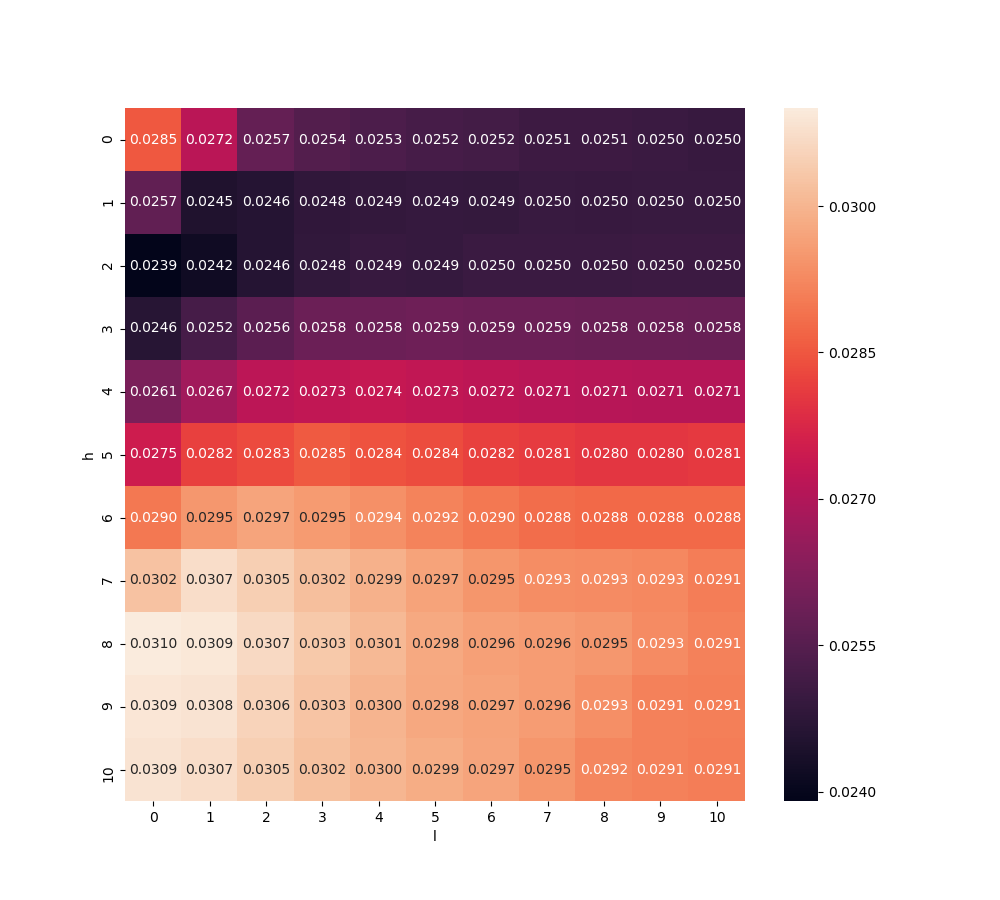
\includegraphics[width=0.6\textwidth,height=\textheight,keepaspectratio]{../result/project2/nmae_heatmap.png}
    \caption{Heat-map of \textsc{NMAE} for each Linear Regressor with $l\in\{0,...,10\}$ when predicting $y^{(t+h)}$}
    \label{fig:1}
\end{figure}

Figure \ref{fig:1} shows us the \textsc{NMAE} of each model when predicting $y^{(t+h)}$. Rows represent the time horizon $h = 0,...,10$ and columns represent the lag $l = 0,...,10$. The color gradient of the heat-map allows us to visualize and extract conclusions better than if we used a normal table.

When we analyze the results by looking at each row we notice that, in most cases, the \textsc{NMAE} decreases as we increase $l$. On the other hand, when we look at each column, we see that the \textsc{NMAE} increases as we increase $h$. Both these events are, intuitively, expected. When we increase $l$, we are providing more information, or context, to the model, so we expect better predictions. When we increase $h$, we are asking for a value that is more distant in time, and so, harder to predict.

This being said, we can also see that, when predicting $h = 1,..,7$, the \textsc{NMAE} don't monotonically decrease, when we increase $l$ from $0$, as expected. An explanation for this might be the fact that we built $11$ different models, as opposed to $11^2$ models, and so $y^{(t+h)}$ predictions are influenced by the noise of unused predictions. Another possible explanation could be that the current state of the system ($l=0$) can better predict the near future ($h>0$) than the actual current state ($h=0$), as system metric variations only have an impact on users after a certain time.

\section*{Task II}
\label{sec:4}

In this task we use a Long Short-Term Memory (LSTM) Network~\cite{LSTM} to target our forecasting problem.

First, we perform the same transformation done in Task I.

We then perform an experiment to study the impact of $l$ on the accuracy of a model and its predictions of $0...10$ steps into the future by building $11$ different models with $l\in\{0,...,10\}$. In this experiment we build stacked LSTM Networks~\cite{SLSTM}, composed of 3 layers. We opted for two LSTM layers as, in our tests, it outperformed networks with a single LSTM layer, while networks with three LSTM layers presented a non-feasible computational overhead. The first layer is an LSTM layer with $100$ units, the second layer is an LSTM layer with $50$ units, while the third and final layer is a Dense layer with $h+1$ units, corresponding to the output. Each model was trained for $100$ epochs, using \texttt{Adam}, with the default learning rate, as the optimization algorithm and the mean-squared error as the loss function. The default values were utilized for all other parameters.

The results can be found below in Figure $\ref{fig:2}$.

\begin{figure}[!ht]
    \centering
    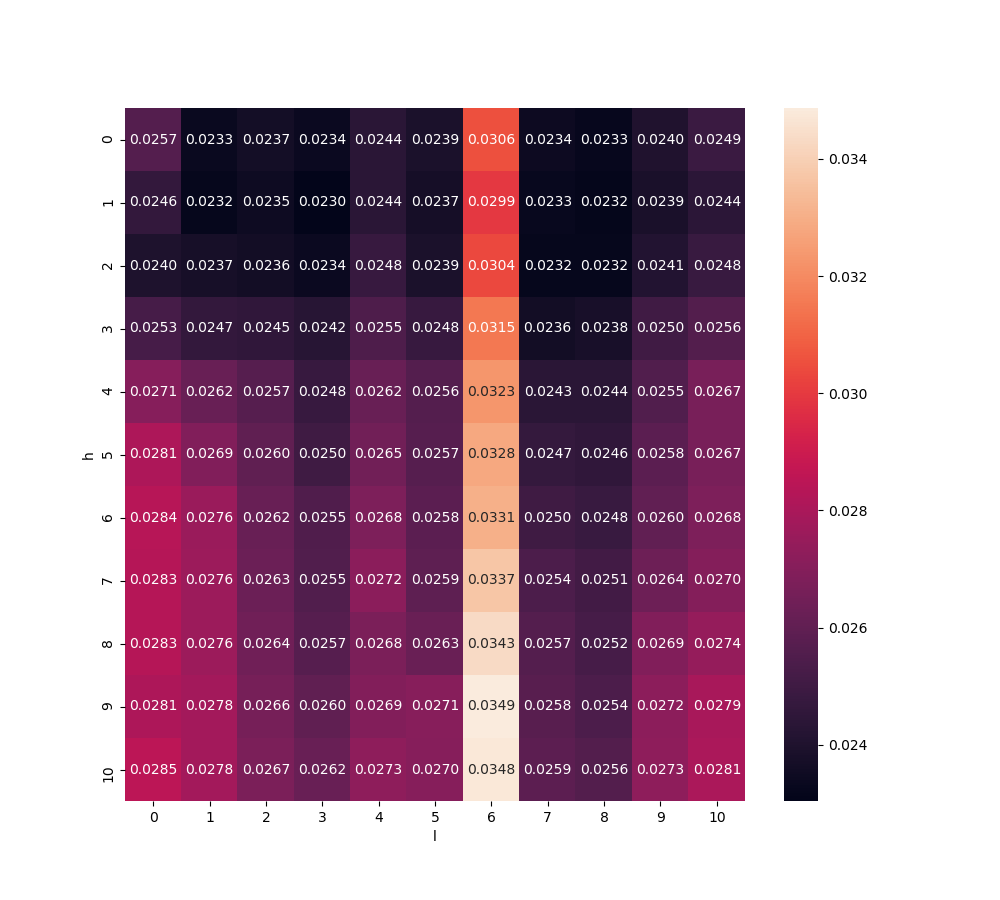
\includegraphics[width=0.6\textwidth,height=\textheight,keepaspectratio]{../result/project2/lstm_nmae_heatmap.png}
    \caption{Heat-map of \textsc{NMAE} for each stacked LSTM~\cite{SLSTM} model with $l\in\{0,...,10\}$ when predicting $y^{(t+h)}$}
    \label{fig:2}
\end{figure}


Figure \ref{fig:2} shows us the \textsc{NMAE} of each model when predicting $y^{(t+h)}$. Rows represent the time horizon $h = 0,...,10$ and columns represent the lag $l = 0,...,10$. The color gradient of the heat-map allows us to visualize and extract conclusions better than if we used a normal table.

When we analyze the results by looking at each row we notice that, in most cases, the \textsc{NMAE} decreases as we increase $l$. On the other hand, when we look at each column, we see that the \textsc{NMAE} increases as we increase $h$. Both these events are, intuitively, expected. When we increase $l$, we are providing more information, or context, to the model, so we expect better predictions. When we increase $h$, we are asking for a value that is more distant in time, and so, harder to predict.

This being said, we can clearly see that the model for $l = 6$ presents very deviated results. This could suggest that, during the training phase, the model hit a local optima or it is overfit, not allowing it to reach the same level of accuracy as the other models.

We can also see that, as in Task I, the \textsc{NMAE} doesn't monotonically decrease as we increase $l$ from 0, as expected. One possible explanation, other than the two, still applicable, explanations suggested in the previous Task, could be related to the training of each model, seeing that each model converges differently.

When comparing these results with the results of Task I, we notice that, in most cases, our \textsc{NMAE}s are lower, which could be explained by the fact that Neural Networks can, theoretically, approximate any given function, which is not the case for Linear Regression.
We can also see that the gradient of the results along the $h$ axis is lower, suggesting that these models can also better forecast than the previous one.

\section*{Task III}
\label{sec:5}

In this task we apply traditional univariate forecasting methods, namely the Autoregression (AR), Moving Average (MA), and Autoregressive Integrated Moving Average (ARIMA) models.

As we will be studying the impact of each of these models given their parameters, as well as the horizon of the predictions, it is useful to also look at a well known method for model identification. 

The autocorrelation (ACF) is a measurement of the correlation between one value and its predecessors. The partial autocorrelation (PACF) is a measurement of the correlation between one value and its predecessors after removing the influence of earlier lags. These are useful tools for better understanding time series, and from where we can extract, for example, information about seasonality and trend. Figures \ref{fig:3} and \ref{fig:4} show us, respectively, the ACF and the PACF, where we can see the respective values for each \textit{lag}, as well as the $95\%$ confidence intervals represented by the light blue funnels.

\begin{figure}[!ht]
    \centering
    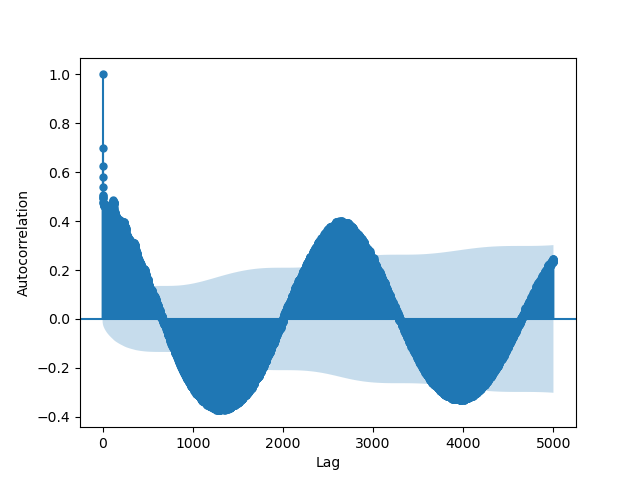
\includegraphics[width=0.40\textwidth,height=\textheight,keepaspectratio]{../acf.png}
    \caption{Plot of the autocorrelation function (ACF) of our time series}
    \label{fig:3}
\end{figure}

\begin{figure}[!ht]
    \centering
    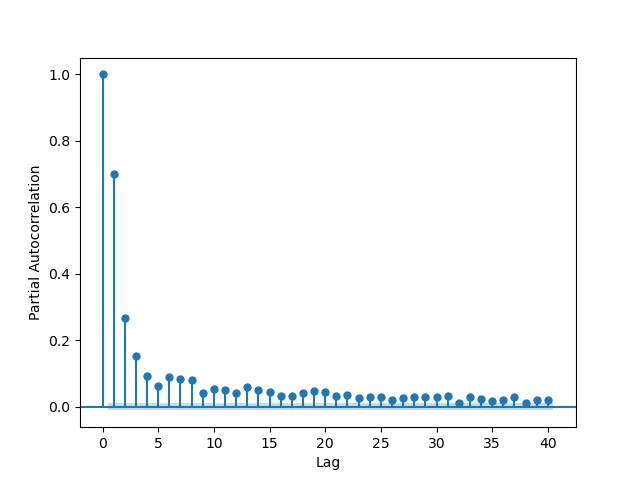
\includegraphics[width=0.40\textwidth,height=\textheight,keepaspectratio]{../pacf.png}
    \caption{Plot of the partial autocorrelation function (PACF) of our time series}
    \label{fig:4}
\end{figure}

Figure \ref{fig:3} shows a clear seasonality in our time series, which can be explained by the way our data was generated in ~\cite{9012741}, following a Poisson process in which the arrival rate is modulated by sinusoidal function.

To perform our experiment, we fit the models with the entirety of the dataset and use the last $30\%$ for our testing. We do this because otherwise it would be difficult to properly test through the \texttt{statsmodels} API. Since we will be studying univariate methods, we only need the target variable, \textit{ReadsAvg}.

To do so, we transform the test set into a list that follows the structure $([y^{(t)},...,y^{(t+h)}],[y^{(t+1)},...,y^{(t+h+1)}],...)$. As we are using analyzing \textit{KV periodic}~\cite{9012741}, our step size (i.e. time between each sample of a sequence), is $1$ second. By using this transformed dataset in our experiments, we are able to conclude on the impact of the parameters $p$ and $q$, as well as compare them with the results from previous tasks.

We then perform an experiment to study the impact of $p$ and $q$ on the accuracy of our models and its predictions of $0...10$ steps into the future by building $10$ different models with $p,q\in\{1,...,10\}$ and calling the \texttt{predict} function for each \texttt{start} and \texttt{end} pair corresponding to each element of the test set. We also need to specify the \texttt{dynamic} parameter to be \texttt{True}, so the prediction uses the forecast values instead of the real observations, which would interfere with our evaluation of the models performance.

Figures \ref{fig:5} and \ref{fig:6} show us the \textsc{NMAE} of each model when predicting $y^{(t+h)}$. Rows represent the time horizon $h = 0,...,10$ and columns represent the lag $p,q = 1,...,10$. The color gradient of the heat-map allows us to visualize and extract conclusions better than if we used a normal table.

\begin{figure}[!ht]
    \centering
    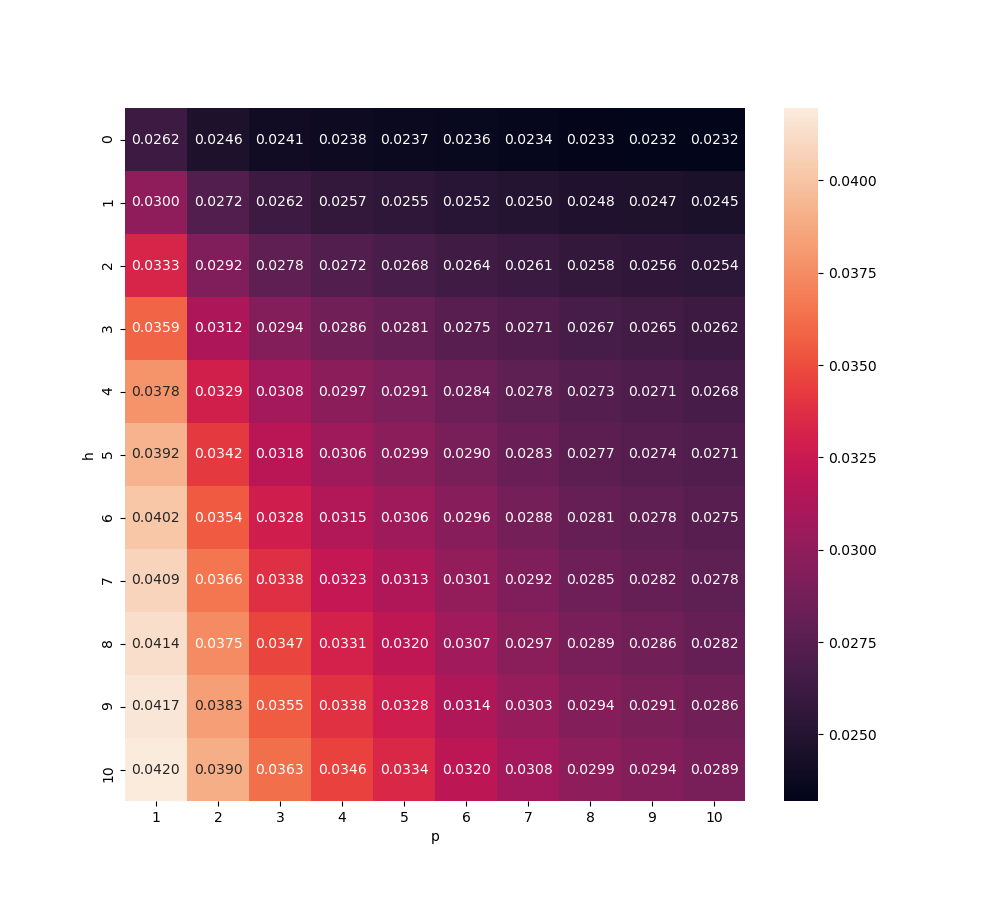
\includegraphics[width=0.6\textwidth,height=\textheight,keepaspectratio]{../ar_nmae_heatmap.png}
    \caption{Heat-map of \textsc{NMAE} for each AR model with $p\in\{1,...,10\}$ when predicting $y^{(t+h)}$}
    \label{fig:5}
\end{figure}


When we analyze the results of Figure \ref{fig:5} by looking at each row, we notice that there is a clear trend in all of them, where the \textsc{NMAE} decreases as we increase $p$. On the other hand, when we look at each column, we see that the \textsc{NMAE} increases as we increase $h$. Both of these events are, intuitively, expected. When we increase $p$, we are utilizing more information, or context, for each prediction, so we expect better predictions. This can also be explained by \ref{fig:3}, where we clearly see that previous results in the considered range of lag have influence in the current state. When we increase $h$, we are asking for a value that is more distant in time, for which the models have to make more assumptions, and so, have a worse accuracy.

We should also note that, even though this model is suitable for series without trend and seasonal components and our series has both, as shown in Figure \ref{fig:3}, it is still able to obtain good results.

\begin{figure}[!ht]
    \centering
    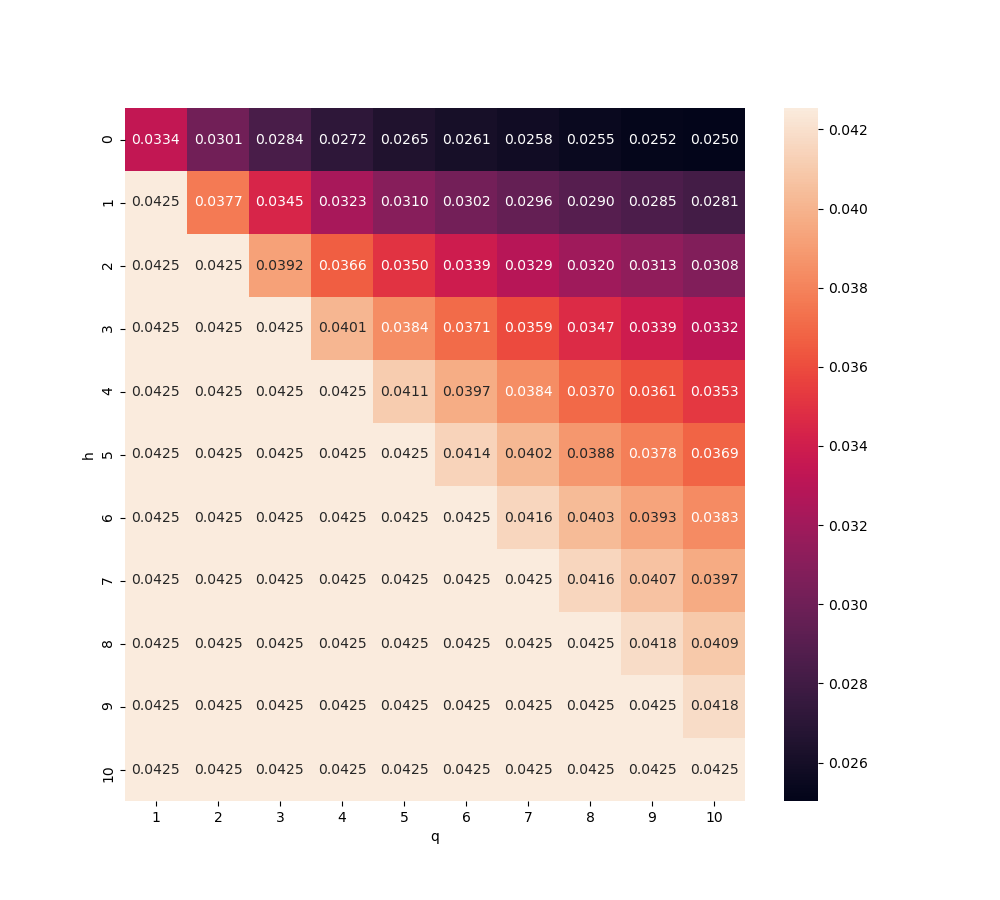
\includegraphics[width=0.6\textwidth,height=\textheight,keepaspectratio]{../ma_nmae_heatmap.png}
    \caption{Heat-map of \textsc{NMAE} for each MA model with $q\in\{1,...,10\}$ when predicting $y^{(t+h)}$}
    \label{fig:6}
\end{figure}

The most noticeable aspect of Figure \ref{fig:6} are the values below the diagonal, where all the results have the same value. This is explained by the definition of the MA model, in which the next value is a linear function of past residual errors. The values below the diagonal represent predictions where $h \geq q$, so all the residual errors utilized are $0$, as this is the value considered during the dynamic prediction, and so the predictions are all equal to the constant values, which, in this case, is equal for every model, as it is the mean of the training set.

When we analyze the results by looking at each column, we notice that the \textsc{NMAE} increases as we increase $h$, even on the upper part of our heat-map. This is, again, explained by the prediction, which, converted to common language, means that we are trying to predict further into the future and, to do so, making more assumptions about the process. 

When we analyze by looking at each row, we are able to see that the \textsc{NMAE} decreases as we increase $q$ which is, again, intuitively explained by the fact that we are taking into account more information and are able, due to this, to better model the real function underneath the process being modeled.

We then study ARIMA, by building 20 different models, 10 with the differentiating factor, $d$, equal to $0$, and 10 with the differentiating factor equal to $1$, and, for each of these, with $p=q\in\{1,...10\}$.

\begin{figure}[!ht]
    \centering
    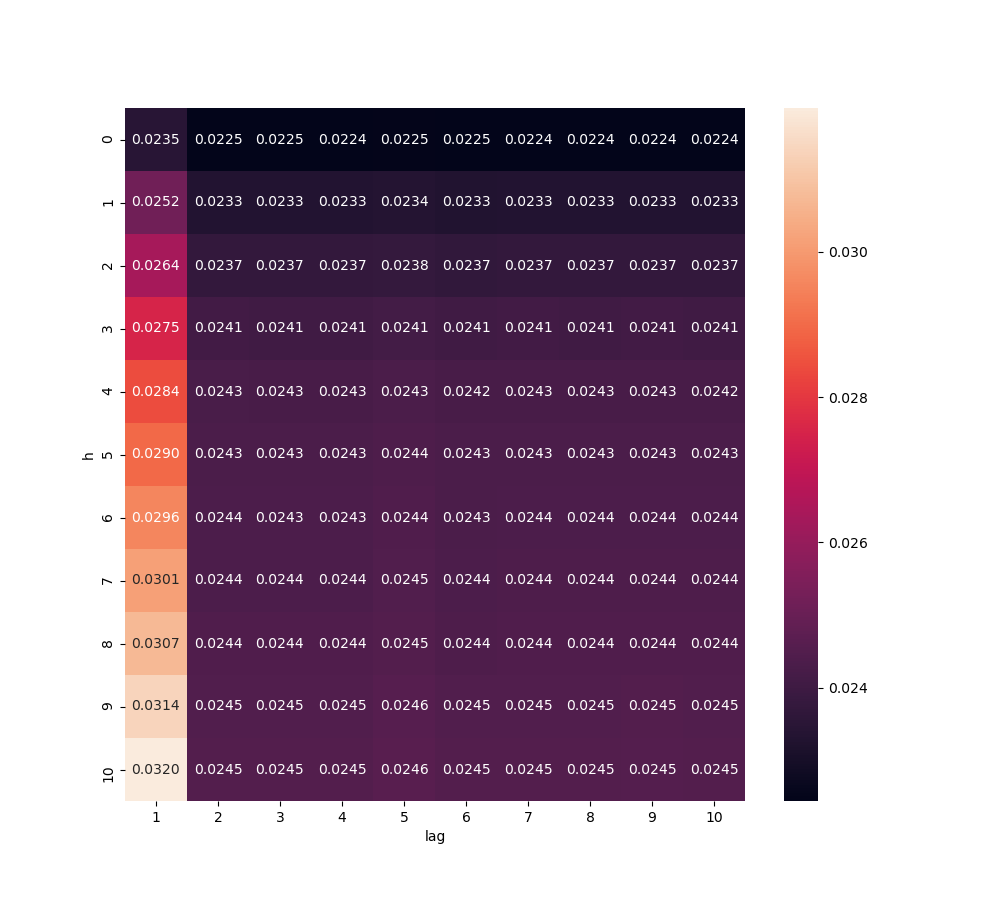
\includegraphics[width=0.6\textwidth,height=\textheight,keepaspectratio]{../arima_d_0_nmae_heatmap.png}
    \caption{Heat-map of \textsc{NMAE} for each ARIMA model with $p=q\in\{1,...,10\}$ and $d=0$ when predicting $y^{(t+h)}$}
    \label{fig:7}
\end{figure}


\begin{figure}[!ht]
    \centering
    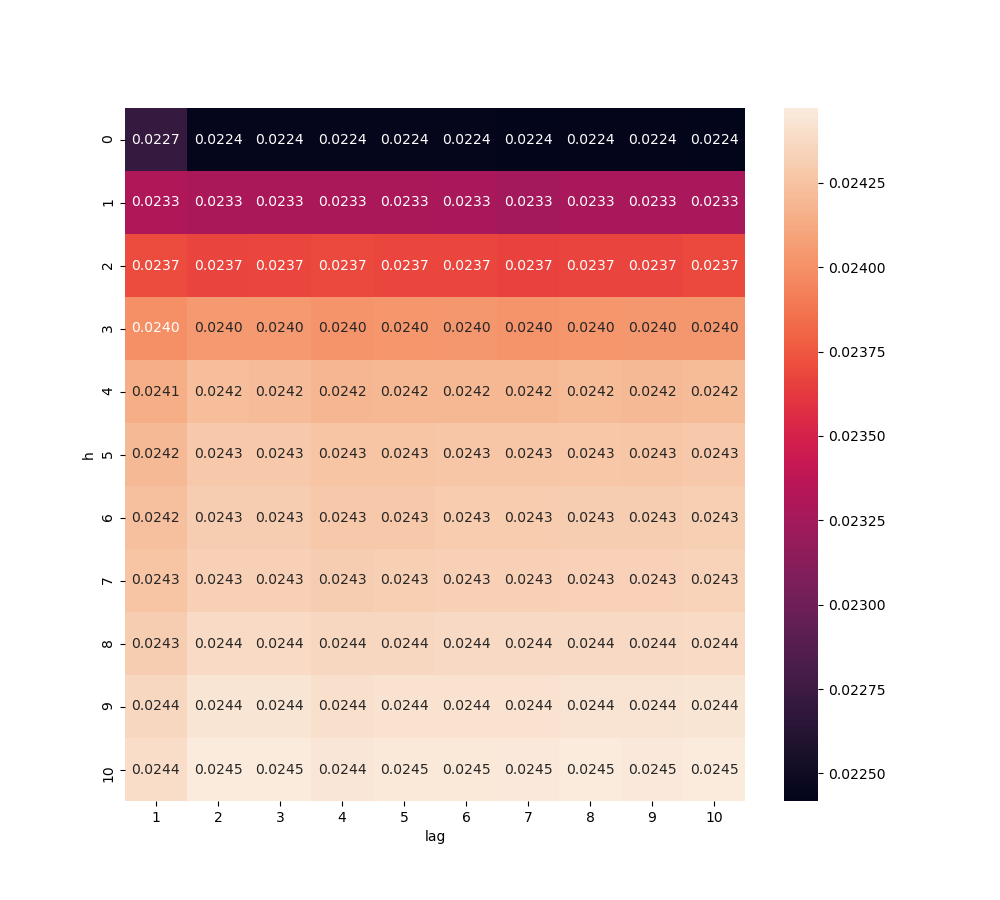
\includegraphics[width=0.6\textwidth,height=\textheight,keepaspectratio]{../arima_d_1_nmae_heatmap.png}
    \caption{Heat-map of \textsc{NMAE} for each ARIMA model with $p=q\in\{1,...,10\}$ and $d=1$ when predicting $y^{(t+h)}$}
    \label{fig:8}
\end{figure}

\pagebreak

We performed experiments for two values of $d$, not just one, as the time series we are analyzing is already stationary.

By looking at Figures \ref{fig:7} and \ref{fig:8}, we can see that, even though our time series is stationary, using the absolute values or the differentiated values results, for almost all values of $lag$, in very similar results. The only exception to this case is the model with $lag=1$ and $d=0$, which deviates from the behavior of other models. We were not able to find a good explanation for this result.

We can also see that, for either value of $d$, all models present a very consistent performance, showing no change, with the exception of the already pointed out model, in the \textsc{NMAE} as we increase the $lag$, and almost no change when increasing $h$, being $h\in\{0,1,2\}$ the standouts.

If we compare the AR and MA models, we can see that the AR model clearly outperforms the MA model. We expected this given the nature of both models. The AR model's order can be evaluated by looking at Figure \ref{fig:4}, which plots the PACF, since this model depends on each lagged value independently of each other. We can see that the PACF converges to values close to $0$ in about $30$ steps. Since the MA model depends on lagged values which are dependent from each other, the ACF is usually a better option for parameter determination. We can clearly see, in Figure \ref{fig:3}, that, contrary to the PACF, the ACF never converges, nor stays stationary around $0$.

By Wold's theorem~\cite{WOLD}, we know that any covariance-stationary time series, such as ours, can be written as the sum of two time series, one deterministic and one stochastic. This means that an ARIMA model, which combines AR (deterministic) and MA (stochastic), can, theoretically, model any time series. By observing the results we got, we notice that our ARIMA models clearly outperform any of the models previously studied. This fact, allied with the consistency of the results across the several combinations of $lag$ and $h$, indicates us that we have found a very close approximation to the real process. The resulting error could be explained by the, relatively, low value of the $q$ parameter in the MA part of the ARIMA model, as explained in the previous paragraph, and the fact that we ignored the seasonality present in out time series.

\section*{Discussion}

In Task I, we studied Linear Regression applied to our forecasting problem and discovered that the results highly depended on the horizon of our predictions, with the models only being competitive for very short horizons.

In Task II, we aimed at improving the previous results by using an LSTM Network. We found that LSTM Networks were better able to fit our process, providing both better results and better consistency over larger horizons.

In Task III, we studied three univariate time series analysis. We found that AR performed better than MA, while the combination of both, along side with differentiation, ARIMA, was the best performing model out of all studied, while demonstrating to be very consistent as we increase the horizon.

Further work on the same topic can include the, more in depth, study of parameters for LSTM Networks, as well as the study of the univariate time series analysis model SARIMA, which adds to ARIMA a seasonality component that could help reach even better results, given the seasonality present in our time series.

\printbibliography

\end{document}
